% -----------------------------------------------
% Template for JIM
%     jim.sty -> style file
% By Eloi Batlle (eloi@iua.upf.es), changes for 
% ICMC by Bram de Jong (bdejong@iua.upf.es)
% changes for JIM 2007 by Dominique Fober (fober@grame.fr)
% changes for JIM 2009 by Olivier Tache (olivier.tache@imag.fr)
% -----------------------------------------------

\documentclass{article}
\usepackage{jim,amsmath}
\usepackage[utf8]{inputenc}
\usepackage[francais]{babel}
\usepackage[T1]{fontenc}
%\usepackage{pxfonts}
\usepackage{graphicx}
\usepackage{color}
\usepackage{hyperref}



% ------------------------------------------------
\newcommand{\inscore}		{\textsc{\small INScore}}
\newcommand{\code}[1]		{\texttt{\small #1}}

\definecolor{mygrey}{gray}{0.93}
\newcommand{\sample}	[1]		{\begin{center}\colorbox{mygrey}{
								\begin{minipage}[t]{0.95\columnwidth} 
								{\small \texttt{#1}}
								\end{minipage}}\end{center}}
\newcounter{excount}
\setcounter{excount}{1}
\newcommand{\exemple}			{\vspace{1mm} \hspace*{-4.5mm}\textbf{Exemple \arabic{excount}} \addtocounter{excount}{1}}


% ------------------------------------------------
% Title.
% ------------------------------------------------
\title{Programmation événementielle de partitions musicales interactives.}
\author{D. Fober, S. Letz, Y. Orlarey\\
{\small \{fober,letz,orlarey\}@grame.fr}\\
Grame - Centre national de création musicale
}

% Single \textsc{address}
% To use with only one author or several with the same address
% ---------------
%\oneauthor
%  {Author} {School \\ Department}

% Two addresses
% --------------
%\twoauthors
%  {First author} {School \\ Department}
%  {Second author} {Company \\ Address}

% Three addresses
% --------------
%\threeauthors
%  {Auteur 1} {Organisme \\ Adresse électronique}
%  {Auteur 2} {Organisme \\ Adresse électronique}
%  {Auteur 3} {Organisme \\ Adresse électronique}

\begin{document}
%
\maketitle
%
\begin{abstract}
\inscore\ est un environnement pour la conception de partitions musicales interactives qui intègre un système original d'interaction basé sur des événements et sur un langage de script permettant d'associer des messages arbitraires à ces événements. Initialement conçu pour être piloté via OSC, la version textuelle des messages OSC s'est rapidement constituée en format de stockage, puis étendue en un langage de script permettant une plus grande souplesse dans la description des partitions et des interactions avec ces partitions. Cet article présente ce langage de script et illustre notamment ses capacités à décrire des interactions sous forme événementielle, tout en restant dans l'espace temporel.
\end{abstract}
%

%----------------------------------------------
\section{Introduction}\label{sec:introduction}

\inscore\ est un environnement pour la conception de partitions musicales qui propose une approche de la notation musicale étendue à des objets graphiques arbitraires \cite{Fober:10c}, incluant la représentation de l'interprétation musicale. Cette approche nouvelle de la notation permet également la représentation des relations temporelles entre les objets de la partition \cite{fober:10b}.

La conception d'\inscore\ fait réponse à une carence des outils informatiques actuels pour la notation de la musique, qui n'ont pas évolué en proportion des nouvelles formes de création musicale (voir par exemple \cite{magnuss11} \cite{freeman11}). 
En particulier, il y a un fossé significatif entre les musiques interactives et la manière statique de les noter.
Les technologies d'aujourd'hui permettent le calcul et l'interaction avec la musique en temps réel, mais la dimension symbolique de la notation est généralement exclue du processus d'interaction excepté dans des travaux très récents \cite{Hoadley12}.

Conçu pour être piloté par des messages OSC \cite{OSC}, \inscore\ se prête naturellement à une utilisation interactive. Cette approche de la programmation de partition par messages est également déclinée en un langage de script, basé sur une extension des messages OSC, et fournissant des primitives d'interaction reposant sur des notions \emph{d'événements}. Ces événements sont similaires à ceux typiquement disponibles pour la gestion des interfaces utilisateurs (par exemple en Javascript via le DOM \cite{dom3ev}), avec une extension dans le domaine temporel.

Cet article présente tout d'abord deux exemples de partitions interactives, mises en oeuvre dans des créations récentes. Il présente ensuite le système de messages et les événements d'interaction, qui permettent à la fois de décrire la partition et d'interagir avec elle. Des exemples d'usages viennent enfin illustrer les capacités d'expression du système. 


%----------------------------------------------
\section{Partitions interactives}

Les musiques interactives sont aujourd'hui l'objet d'intérêts artistiques et scientifiques convergents. L'interaction soulève des problèmes à la fois pour la composition, la description et pour l'exécution des oeuvres. Ces problèmes sont abordés dans les aspects temporels de la partition interactive \cite{allombert09} ou du contrôle \cite{acont08}, et sont liés au calcul de l'oeuvre.

Pour la notation de l'oeuvre interactive, deux créations récentes ont mis en oeuvre \inscore\ pour créer des partitions dynamiques avec des approches originales, qui témoignent également des besoins de la création contemporaine. Il s'agit de \emph{Calder's Violin} et de \emph{Alien Lands}.

\subsection{Calder's Violin}
\textit{Calder's violin}, composé par Richard Hoadley, a été créé à Cambridge en Octobre 2011. La pièce est définie comme \emph{"musique automatique pour violon et ordinateur"} et présente dynamiquement au musicien, de la notation musicale symbolique générée de manière algorithmique (figure \ref{fig:cv}). Cette partition est alors jouée par le musicien en parallèle des sons générés par l'ordinateur ou par d'autres musiciens. Les technologies utilisées reposent sur SuperCollider pour l'environnement de programmation audio et sur \inscore\ pour la notation. Pour plus de détails se référer à \cite{Hoadley12}. 

\begin{figure}[htbp]
\centerline{
	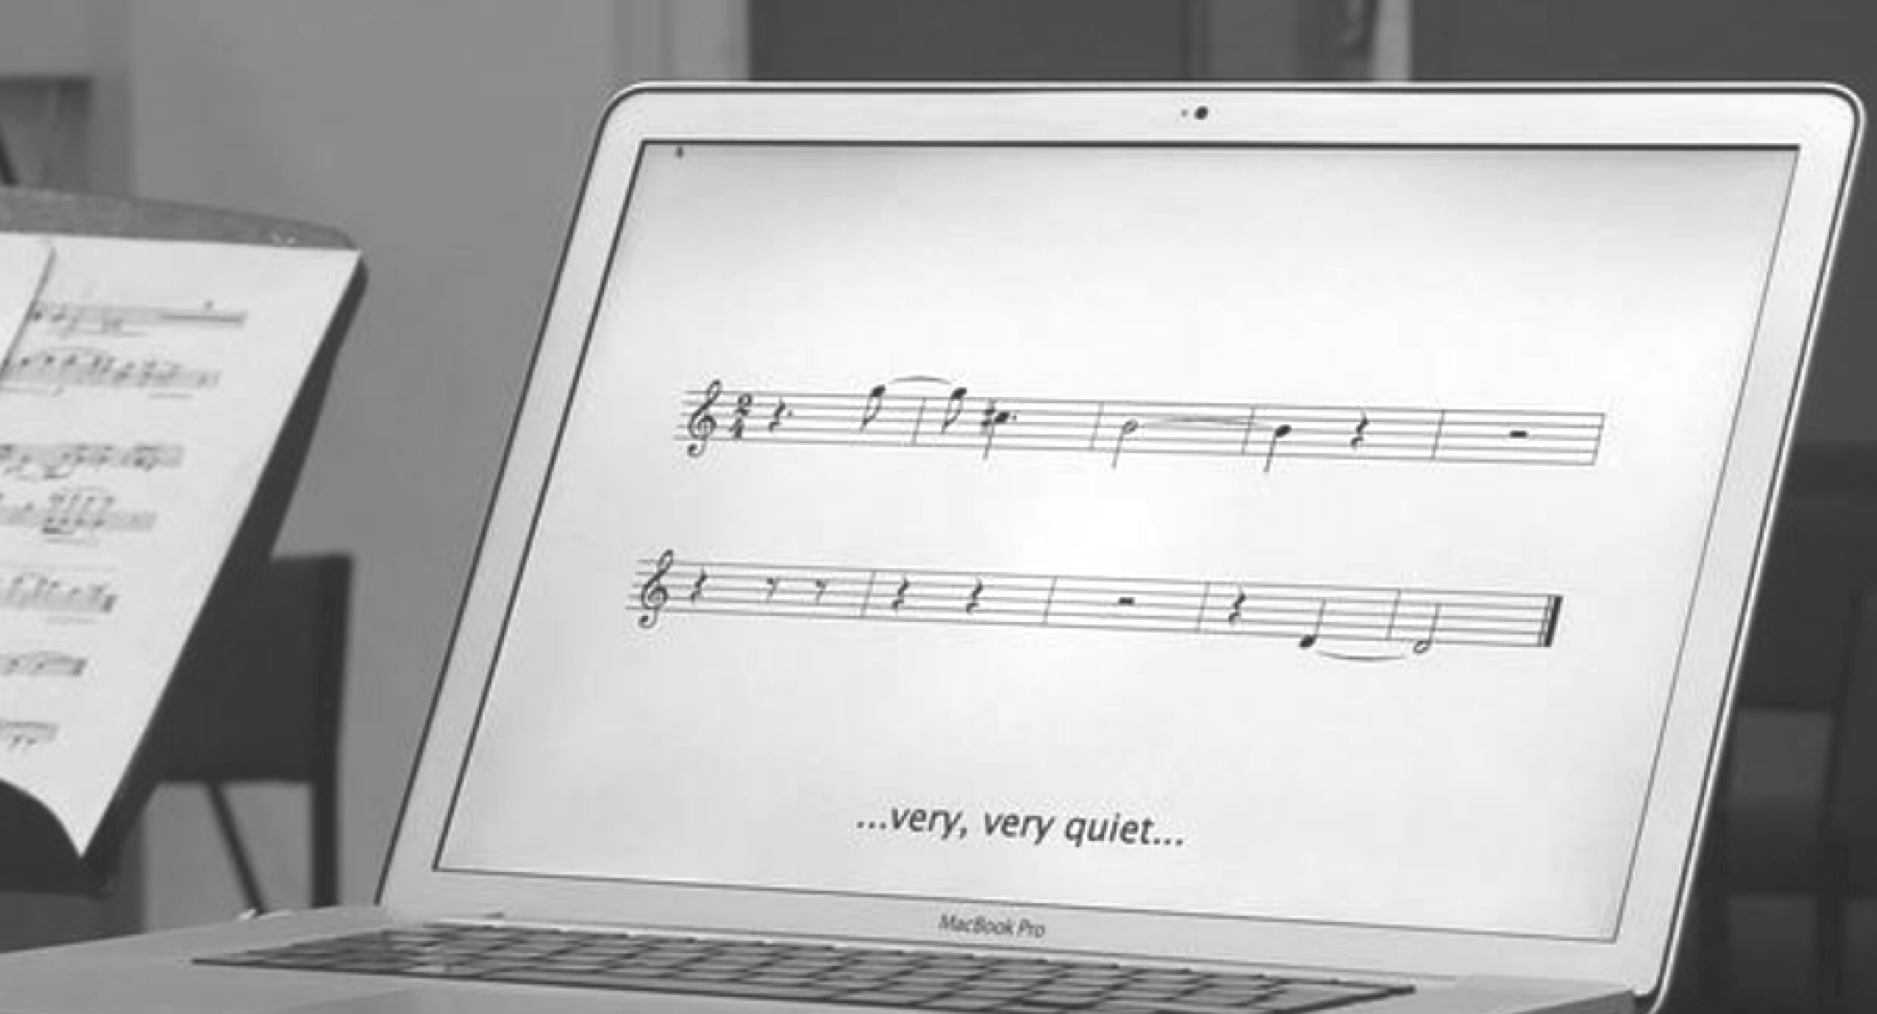
\includegraphics[width=0.9\columnwidth]{imgs/caldersv}}
\caption{Calder's Violin : exemple de partition.}
\label{fig:cv}
\end{figure}


\subsection{Alien Lands}

\textit{Alien Lands} est un ensemble de pièces pour percussions et quatuor à corde, composées par Sandeep Bhagwati. Dans leur version interactive, ces pièces ont été données à Montreal en Février 2011.
L'utilisation d'\inscore\ relève de quatre catégories:
\begin{itemize}
\item partition traditionnelle avec tourne de page automatique,
\item partition avec choix automatiques réalisés par l'ordinateur : ordre des mesures, sélection de lignes,
\item partition complexe automatique, comprenant des éléments générés de manière algorithmique (figure \ref{fig:al}),
\item partition complexe interactive, où les éléments algorithmique sont générés à la demande des musiciens.
\end{itemize}

\begin{figure}[htbp]
\centerline{
	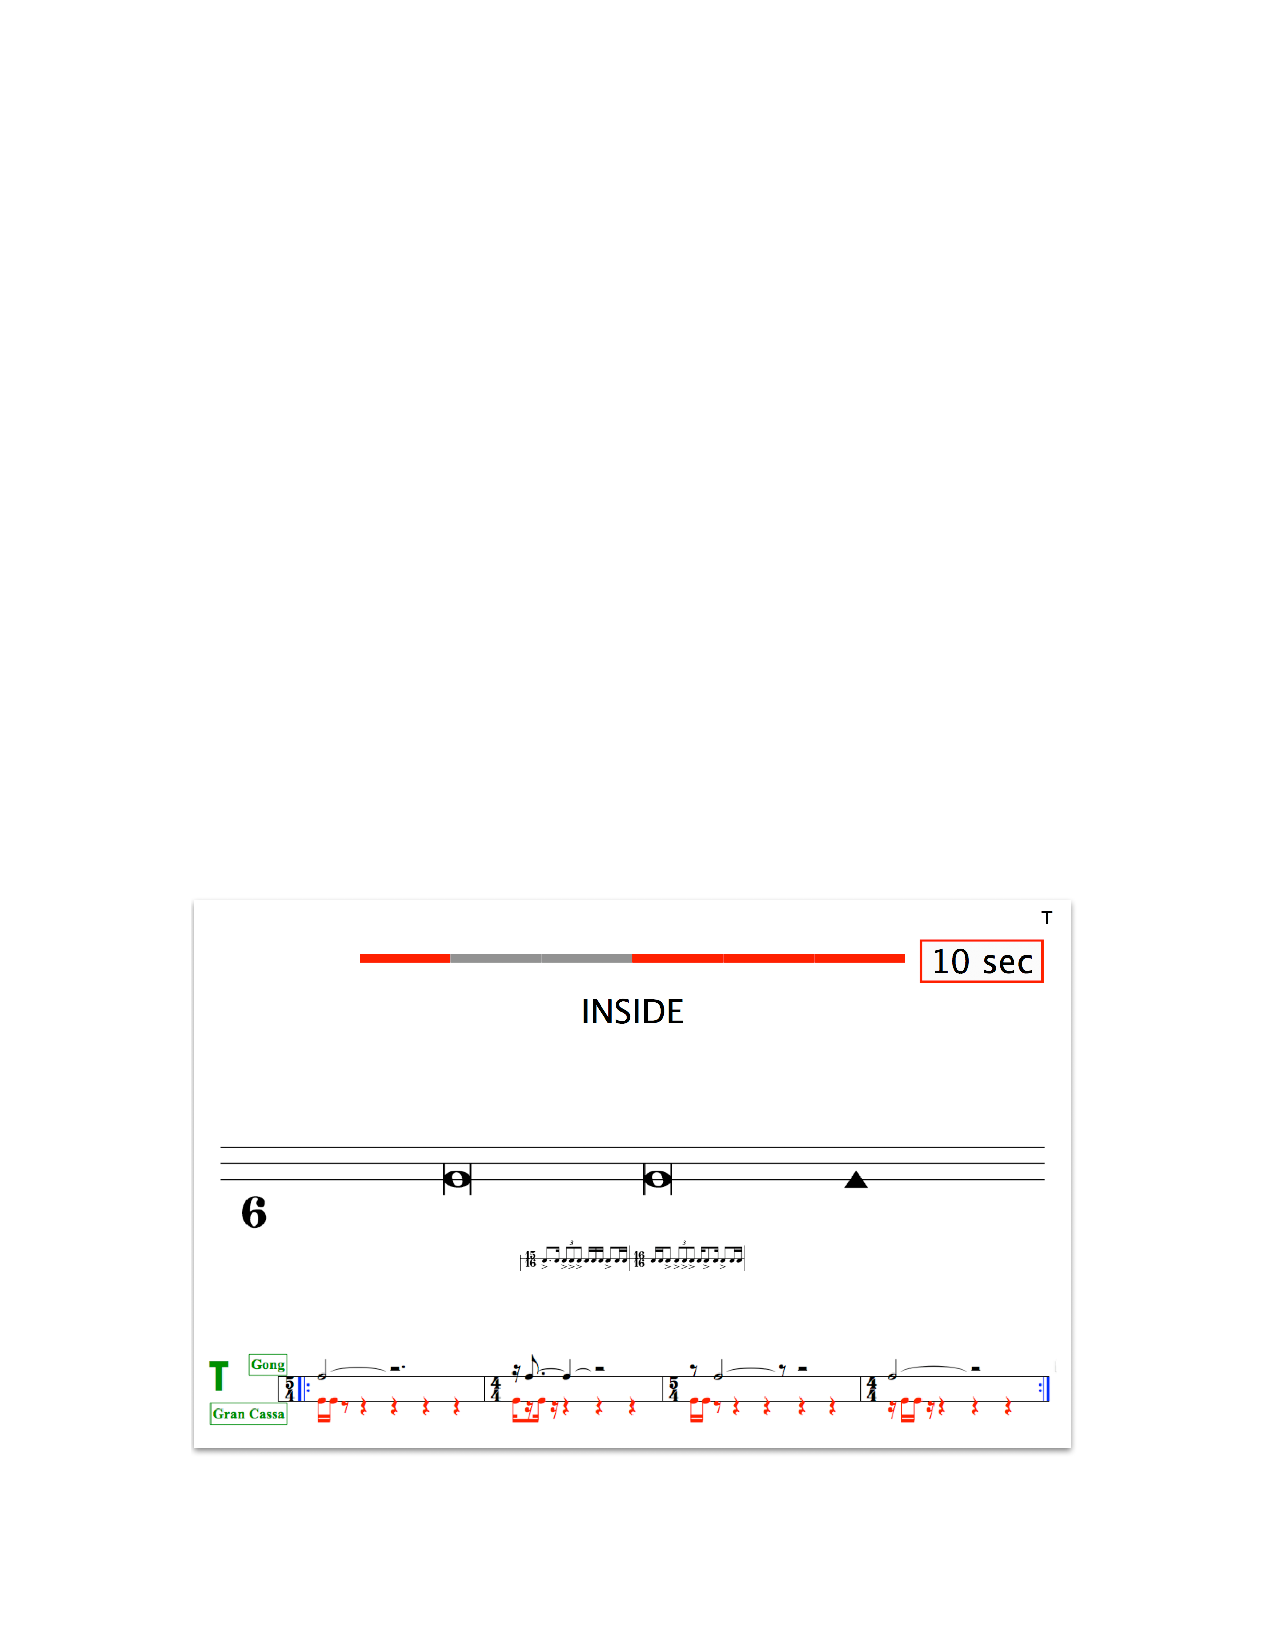
\includegraphics[width=0.94\columnwidth]{imgs/alienscore}}
\caption{Alien Lands : une partition complexe automatique.}
\label{fig:al}
\end{figure}


%----------------------------------------------
\section{Design de partition par messages}\label{sec:msgs}

Le principe de base pour la description d'une partition, consiste à envoyer des messages OSC au système pour créer les différents composants de la partition et pour contrôler leurs attributs, aussi bien dans l'espace graphique que temporel.

%========================
\subsection{Format général des messages}
Le format général des messages \inscore\ est illustré figure \ref{fig:fgal}. Il s'agit d'une spécialisation des messages OSC qui peut être vue comme \emph{orientée objet}, où l'adresse désigne l'objet cible du message, \code{method} désigne une méthode de l'objet cible et \code{params}, les paramètres de la méthode.
Un message \inscore\ peut donc être vu comme l'appel d'une méthode d'un objet de la partition.


\begin{figure}[htbp]
\centerline{
	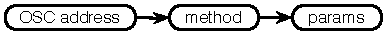
\includegraphics[width=0.8\columnwidth]{imgs/formatgal}}
\caption{Format général des messages INScore.}
\label{fig:fgal}
\end{figure}

Le système inclut des messages pour gérer les attributs graphiques des composants de la partition (position, couleur, échelle, rotations, effets...), pour gérer leurs attributs temporels (date, durée), pour exprimer les relations entre espaces graphiques et temporels, pour synchroniser des objets, pour représenter des signaux et pour gérer des événements d'interaction.

\exemple  Change la position \code{x} de l'objet \code{obj}. L'adresse décrit la hiérarchie des objets : \code{obj} est contenu dans une scène nommée \code{scene} qui est incluse dans l'application d'adresse \code{ITL}.
\vspace{-1mm}\sample{/ITL/scene/obj x -0.5}


%========================
\subsection{Le langage de script}

Bien que prévu pour être émis sous forme de paquets sur un réseau, les messages OSC peuvent s'exprimer sous forme textuelle. C'est cette forme textuelle qui constitue le format de sauvegarde des partitions. Elle a été rapidement étendue pour en faire un langage de script.

\subsubsection{Adresses étendues}
Les adresses OSC sont étendues pour permettre l'émission de messages aussi bien vers \inscore\ qu'à destination d'une machine et/ou application externes (figure \ref{fig:eaddr}). Cela permet d'initialiser à la fois la partition et les ressources externes qui peuvent y être associées.

\begin{figure}[htbp]
\centerline{
	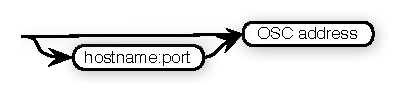
\includegraphics[width=0.8\columnwidth]{imgs/extaddress}}
\caption{Extension du schéma d'adressage.}
\label{fig:eaddr}
\end{figure}

\exemple  Initialisation d'une partition et d'une application externe à l'écoute du port 12000, sur une machine nommée \code{host.adomain.net}. Dans les scripts, le point virgule (;) est utilisé comme terminaison de message.
\vspace{-1mm}\sample{/ITL/scene/score set gmnf 'myscore.gmn'; \\
host.adomain.net:12000/run 1; }


\subsubsection{Variables}

Des variables ont été introduites pour permettre le partage de paramètres entre messages. Une variable associe un identificateur et une liste de paramètres ou une liste de messages (figure \ref{fig:var}). Les variables peuvent être utilisées dans les paramètres des messages sous la forme \code{\$identificateur}.

\begin{figure}[htbp]
\centerline{
	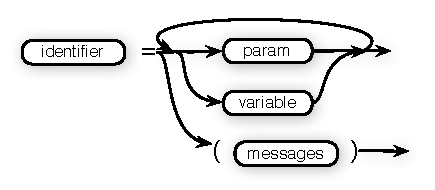
\includegraphics[width=0.8\columnwidth]{imgs/variables}}
\caption{Variables.}
\label{fig:var}
\end{figure}

\exemple  Déclaration de variables et utilisation comme paramètre de couleur. Le caractère '!' marque le début d'un commentaire.
\vspace{-1mm}\sample{color = 200 200 200; \\
colorwithalpha = \$color 100;\\
msgsvar= ( ! une liste de messages\\
\hspace*{3mm}localhost:7001/world "Hello world",\\ 
\hspace*{3mm}localhost:7001/world "how are you ?" ); \\ 
/ITL/scene/obj color \$colorwithalpha;
 }

\subsubsection{Langages}

Les scripts supportent également l'inclusion de langages de programmation comme javascript (par défaut) ou lua. Les sections correspondantes sont indiquées de manière similaire à html (figure \ref{fig:lang}). Le code est évalué au moment de la lecture du script et le résultat attendu de l'évaluation est un ensemble de messages \inscore\ qui vont remplacer le script correspondant.

\begin{figure}[htbp]
\centerline{
	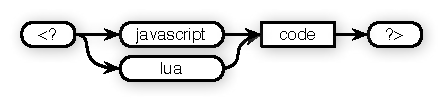
\includegraphics[width=0.8\columnwidth]{imgs/scripts}}
\caption{Langages.}
\label{fig:lang}
\end{figure}


%----------------------------------------------
\section{Interaction événementielle}\label{sec:interaction}

Le processus d'interaction événementielle repose sur l'association de messages à des événements du système. Ces messages sont émis lorsque l'événement auquel ils sont associés se produit. Le format général des messages pour créer de telles associations est décrit en figure \ref{fig:watch}.

\begin{figure}[htbp]
\centerline{
	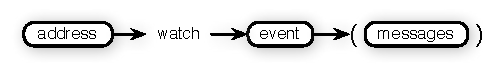
\includegraphics[width=0.95\columnwidth]{imgs/watch}}
\caption{Format général d'un message d'interaction.}
\label{fig:watch}
\end{figure}


%----------------------------------------------
\subsection{Typologie des événements}\label{subsec:typologie}

Les événements définis par le système sont d'une part des événements typiques d'interface utilisateur (tels que clics de souris par exemple) ainsi que des événements définis dans le domaine temporel (table \ref{tbl:evts})

\begin{table}[htdp]
\begin{center}
\begin{tabular}{c|c}
Domaine graphique & Domaine temporel \\
\hline
mouseDown 		& timeEnter	\\
mouseUp			& timeLeave	\\
mouseEnter		& durEnter		\\
mouseLeave		& durLeave		\\
mouseMove		&				\\
\end{tabular}
\end{center}
\caption{Principaux événements du système.}
\label{tbl:evts}
\end{table}%

Dans le domaine temporel, un événement est déclenché quand un objet entre ou quitte une zone temporelle (\code{timeEnter, timeLeave}) définie par deux dates, ou quand la durée d'un objet entre ou quitte une zone temporelle (\code{durEnter, durLeave}) définie par deux durées.


%----------------------------------------------
\subsection{Variables contextuelles}
Lorsqu'un événement se produit, les messages associés sont évalués, notamment parce qu'ils peuvent faire référence à des \emph{variables contextuelles}. Ces variables concernent principalement les événements du domaine graphique et permettent d'accéder à la position de la souris au moment de l'événement dans différents référentiels (\code{\$x \$y \$sx \$sy}) ou encore à la date correspondant à cette position (\code{\$date}).

\exemple   Un objet qui suit les clics de la souris. La virgule (,) est utilisée comme séparateur de message dans les listes de messages.
\sample{/ITL/scene/obj watch mouseDown (\\
\hspace*{12mm}/ITL/scene/obj x '\$sx', \\
\hspace*{12mm}/ITL/scene/obj y '\$sy' );}



%----------------------------------------------
\section{Cas d'usage}\label{sec:exemples}


%----------------------------------------------
\subsection{Tourne de page} \label{pageturn}

Une application simple des événements temporels con-siste à décrire des tournes de page automatique. Un objet surveille les zones temporelles correspondants aux différentes pages et rappelle ces pages lorsque qu'il entre dans ces zones. A noter que cet objet peut aussi bien être un curseur qui se déplace sur la partition.
\sample{/ITL/scene/obj watch timeEnter 0 12	\\
\hspace*{25mm}(/ITL/scene/score page 1);	\\
/ITL/scene/obj watch timeEnter 12 24	\\
\hspace*{25mm}(/ITL/scene/score page 2);	\\
\hspace*{1mm}etc.
}

%----------------------------------------------
\subsection{Séquences d'interactions} \label{seqitl}

Les messages d'interaction décrits en figure \ref{fig:watch} acceptent des messages arbitraires du système en tant que messages associés à un événement. Il est donc possible d'associer un message d'interaction à un événement et ainsi, de décrire des séquences d'interactions.

\exemple   Description d'une séquence d'interactions basées sur le clic de souris : le premier clic change la couleur de l'objet, le second modifie l'échelle, le troisième fait une rotation, le quatrième modifie également l'échelle. La profondeur de ces associations n'est pas limitée. 
\sample{/ITL/scene/obj watch mouseDown ( 		\\
\hspace*{4mm}/ITL/scene/obj color 100 100 255,	\\
\hspace*{4mm}/ITL/scene/obj watch mouseDown (		\\
\hspace*{8mm}/ITL/scene/obj scale 1.4,			\\
\hspace*{8mm}/ITL/scene/obj watch mouseDown ( \\
\hspace*{12mm}/ITL/scene/obj angle 45. ,	 \\
\hspace*{12mm}/ITL/scene/obj watch mouseDown ( \\
\hspace*{16mm}/ITL/scene/obj scale 0.8 ))));
}


%----------------------------------------------
\subsection{Séquences dans le domaine temporel}

La séquence d'interactions décrites ci-dessus (section \ref{seqitl}) peut se décliner dans le domaine temporel en associant les changements d'état à des événements temporels et en déplaçant l'objet dans le temps. Avec cette approche, il est à la fois possible de changer l'ordre des événements, mais également de contrôler le déroulement de ces événements dans le temps.

Ce type de description permet de combiner dans une même expression, des approches événementielles, des accès non-séquentiel et du contrôle temporel.

\exemple   Description d'une séquence d'interactions par association à des événements temporels. Les événements temporels sont déclenchés par l'entrée de l'objet dans des zones temporelles consécutives, et dont la durée est la ronde. 
\sample{/ITL/scene/obj watch timeEnter 1 2	\\
\hspace*{10mm}(/ITL/scene/obj color 100 100 255);	\\
/ITL/scene/obj watch timeEnter 2 3	\\
\hspace*{10mm}(/ITL/scene/obj scale 1.4);	\\
/ITL/scene/obj watch timeEnter 3 4	\\
\hspace*{10mm}(/ITL/scene/obj angle 45.);	\\
/ITL/scene/obj watch timeEnter 4 5	\\
\hspace*{10mm}(/ITL/scene/obj scale 0.8);
}


%----------------------------------------------
\subsection{Structuration de l'espace temps}
Dans le cadre d'expériences pédagogiques réalisées aux Ateliers des Feuillantines, la reconstruction du canon par ton de l'Offrande Musicale de J.S. Bach a été réalisée sous forme d'un objet à la fois \emph{partition et instrument}, et \inscore\ a été utilisé pour calculer dynamiquement la représentation symbolique de la musique jouée \footnote{{\scriptsize \url{http://tinyurl.com/ah3jftu}}}. 
L'objet réalisé représente la structure de l'oeuvre en trois dimensions (figure \ref{fig:offr}). Chaque barreau, sur lequel un capteur peut être posé, est muni d'une étiquette indiquant le chemin a suivre, et correspond à une transposition du canon.

\begin{figure}[htbp]
\centerline{
	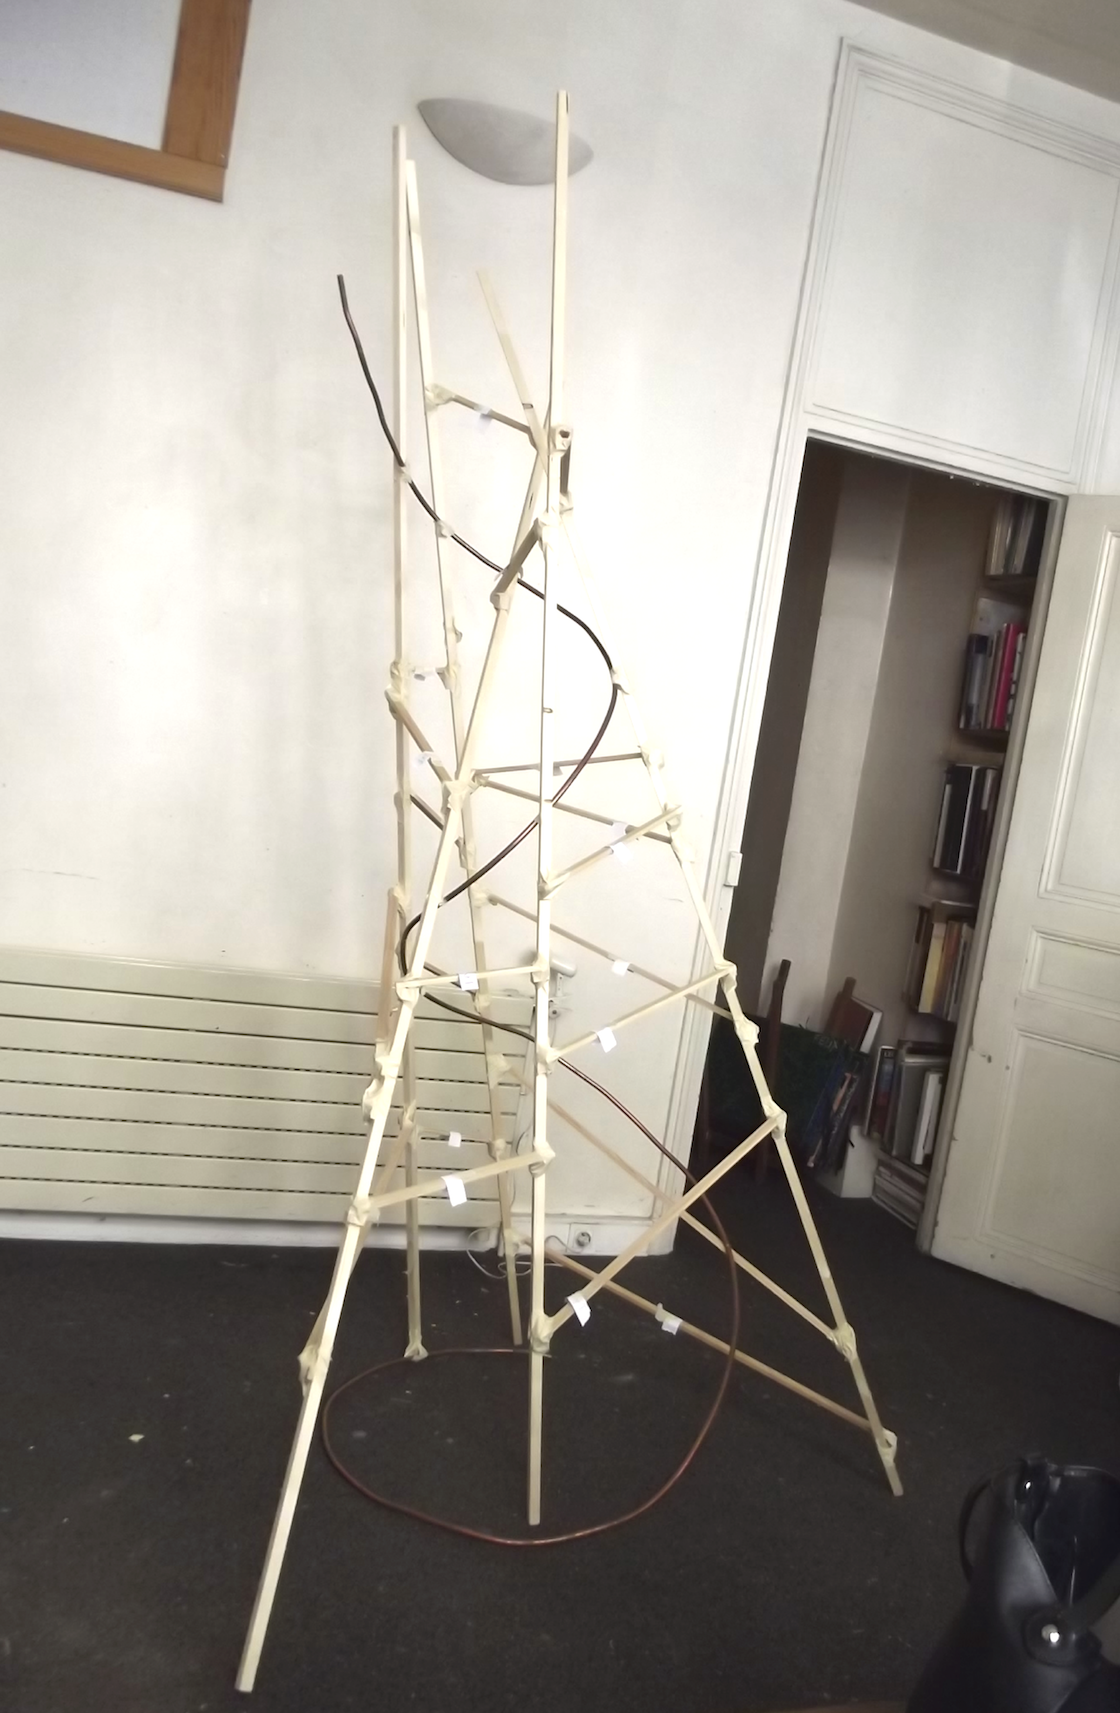
\includegraphics[width=0.5\columnwidth]{imgs/offrande}}
\caption{L'objet \emph{partition / instrument} de l'Offrande musicale.}
\label{fig:offr}
\end{figure}

Du point de vue de la représentation symbolique, les différentes transpositions peuplent l'espace temporel à des dates différentes, de telle sorte que sur l'instrument, l'association d'une position à une date permet de rappeler la transposition correspondante via les événements temporels d'\inscore.


%----------------------------------------------
\section{Conclusion}\label{sec:conclusion}

L'association de messages à des événements se révèle être un mécanisme simple, puissant et homogène pour la description de partitions dynamiques. Il est désormais possible de décrire l'ensemble des comportements d'une partition dans le langage de script d'\inscore . L'utilisation d'applications externes pour piloter ces comportements peut dès lors se limiter au déplacement d'objets dans le temps en associant à ces objets, des comportements liés à des espaces temporels.


%=============================================================
\vspace{4mm}
\hspace{-5mm}
\textbf{Remerciements} \\
Cette recherche a été menée dans le cadre du projet \mbox{INEDIT} qui est soutenu par l'Agence Nationale pour la Recherche [ANR-12-CORD-009-03].

%\bibliographystyle{unsrt}
\bibliographystyle{IEEEtranS}
\bibliography{../interlude}

\end{document}
